\documentclass[12pt,a4paper]{article}
\usepackage[utf8]{inputenc}
\usepackage{amsmath}
\usepackage{amsfonts}
\usepackage{amssymb}
\usepackage[margin=2.5cm]{geometry}
\usepackage{graphicx}
\usepackage{caption}
\usepackage{subcaption}
\usepackage[nottoc,numbib]{tocbibind}
\title{Physical Properties of Zener Tunnelling Nano-devices in Graphene: Supplementary Information}
\author{R. D. Y. Hills and F. V. Kusmartsev}
\begin{document}
%%%%%
%%%%%
%%%%%
%%%%%
%%%%%
\maketitle
	\section{Supplementary Information}
	Here we present supplementary information for the paper titled "Physical Properties of Zener Tunnelling Nano-devices in Graphene". The information here provides additional derivation for the calculations in the main text, which may be of interest to the reader.
		\section{Landauer Formalism in Graphene}
			In this section the Landauer formalism is derived for a graphene scattering device. For a single channel system at non-zero temperatures the current through the system shown in Figure \ref{introduction-current} can be found [28].
			\begin{figure}[h]
				\centerline{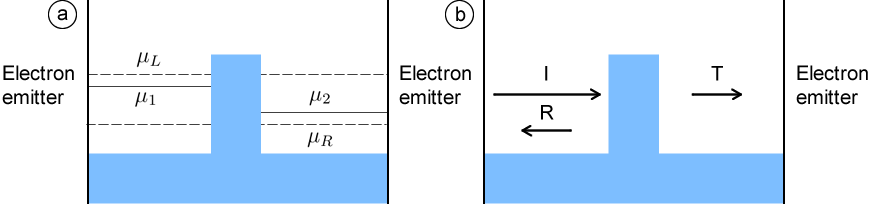
\includegraphics[scale=0.5]{current}}
				\caption{(Colour Online) (a) Diagram showing quasi-Fermi-energies and chemical potentials of the perfectly conducting wires. Here the left emitter injects electrons up to the quasi-Fermi-energy $\mu_{L}$ and the right emitter injects electrons up the the quasi-Fermi-energy $\mu_{R}$. $\mu_{1}$ and $\mu_{2}$ are the chemical potentials of the perfectly conducting wires to the left and right of the scattering device. (b) A scattering device between two electron emitters. Charge carriers from the left emitter are scattered with a probability $R$ of being reflected and probability $T$ or transmitting through the scattering device.}
				\label{introduction-current}
			\end{figure}
			 The system in Figure \ref{introduction-current} consists of 2 incoherent electron reservoirs, which emit charge carriers up to the quasi-Fermi-energy $\mu_{L,R}$, where the subscript $L$ and $R$ represent the reservoir at left or right side of the system respectivly. These reservoirs are then connected to a scattering device via perfect and identical one dimensional conductors. These conductors have chemical potentials $\mu_{1}$ and $\mu_{2}$. The current leaving the left reservoir is then:
			\begin{equation}
				I=ev_{f}\frac{dn}{dE}\left(\mu_{L}-\mu_{R}\right)
				\label{current-dos}
			\end{equation}
			where $e$ is the electron charge, $v_{f}$ is the Fermi velocity and $dn/dE$ is the density of states. The current that is transmitted through the sample is then:
			\begin{equation}
				I=ev_{f}\frac{dn}{dE}T\left(\mu_{R}-\mu_{R}\right)
				\label{current-transmit}
			\end{equation}
			where $T$ is the transmission probability through the scattering device. In [11] the density of states for a single unit cell of graphene at a Dirac point is given by:
			\begin{equation}
				\frac{dn}{dE}=\frac{2A_{c}}{\pi}\frac{|E|}{\hbar^{2}v_{f}^{2}}
				\hspace{1cm}
				A_{c}=\frac{3\sqrt{3}a^{2}}{2}
			\end{equation}
			We define $L_{x}L_{y}/A_{c}$ as the number of unit cells in the sample, where  $L_{x}, L_{y}$ is the size of the sample in the respective dimension. The quantity $L_{x}L_{y}/A_{c}$ shows how many graphene unit cells are present in our sample. As only the $x$-direction current will be considered here, the current in the $x$-direction will be the same in each cell, therefore only the number of graphene unit cells in the $y$-direction will affect the $x$-directional current. This way the quantity $L_{x}$ can be set to one and removed from the calculation. The current through the graphene sample from equation (\ref{current-transmit}) in the $x$-direction becomes:
			\begin{equation}
				I_{x}=e\frac{2L_{y}}{\pi \hbar^{2}v_{f}}T\left(E,\theta\right)\left(\mu_{L}-\mu_{R}\right)|E|cos\left(\theta\right)
			\end{equation}
			The energy and theta dependence for $T$ has been included here to allow for the graphene transmission probability. At non-zero temperatures the states are instead filled according to the corresponding Fermi-Dirac distribution.
			\begin{equation}
				f\left(E-\mu_{L,R}\right)=\frac{1}{e^{\frac{E-\mu_{L,R}}{k_{b}t}}+1}
			\end{equation}
			The current must then be integrated over all energies to account for all states in the Fermi-Dirac distributions.
			\begin{equation}
				I_{x}=I_{0}\int^{\infty}_{-\infty}\int^{\pi/2}_{-\pi/2}T\left(E,\theta\right)\left[f\left(E-\mu_{L}\right)-f\left(E-\mu_{R}\right)\right]|E|cos\left(\theta\right)dEd\theta
			\end{equation}
			with the constant $I_{0}=e\frac{2L_{y}}{\pi\hbar^{2}v_{f}}$. This result for current can then be used with the definition of conductance, $G=I/V$ to find the conductance at a finite temperature for graphene. The potential difference $V$ is determined by the number of charges on the left and right of the scattering device. This can be found by considering the chemical potentials of the perfectly conducing wires. The chemical potentials $\mu_{1,2}$ must be between the quasi-Fermi-energies of the electron emitters $\mu_{L,R}$. The positioning of these chemical potentials requires that the number of occupied states (electrons) above $\mu_{1}$ is equal to the number of unoccupied states (holes) below $\mu_{1}$, and likewise for states above and below $\mu_{2}$. As all states below $\mu_{R}$ must be filled, only the energy range between $\mu_{L}$ and $\mu_{R}$ needs to be considered. Allowing for positive and negitive velocities the number of states between this range is $2\left(dn/dE\right)\left(\mu_{L}-\mu_{R}\right)$. To the right of the scattering device the number of occupied states is the total number of states available in the wire multiplied by the transmission probability; $T\left(dn/dE\right)\left(\mu_{L}-\mu_{2}\right)$. The number of unoccupied states must therefore be the total number of states available in the wire minus the filled states $\left(2-T\right)\left(dn/dE\right)\left(\mu_{2}-\mu_{R}\right)$. As the number of occupied states is equal to the number of unoccupied states we can write:
			\begin{equation}
				T\left(dn/dE\right)\left(\mu_{L}-\mu_{2}\right)=\left(2-T\right)\left(dn/dE\right)\left(\mu_{2}-\mu_{R}\right)
				\label{mu-2}
			\end{equation}
			On the left of the scattering device the number of occupied states includes those filled by incident and reflected charge carriers $\left(1+R\right)\left(dn/dE\right)\left(\mu_{L}-\mu_{1}\right)$. The number of unoccupied states is then $\left(2-\left(1+R\right)\right)\left(dn/dE\right)\left(\mu_{1}-\mu_{R}\right)$. The number of occupied and unoccupied states must be equal, therefore:
			\begin{equation}
				\left(1+R\right)\left(dn/dE\right)\left(\mu_{L}-\mu_{1}\right)=\left(2-\left(1+R\right)\right)\left(dn/dE\right)\left(\mu_{1}-\mu_{R}\right)
				\label{mu-1}
			\end{equation}
			The potential difference between the two wires caused by the scattering device is then:
			\begin{equation}
				eV=\mu_{1}-\mu_{2}
			\end{equation}
			Using equations (\ref{mu-2}) and (\ref{mu-1}) the potential difference across the sample is then:
			\begin{equation}
				eV=R\left(\mu_{L}-\mu_{R}\right)
			\end{equation}
			However, at non-zero temperatures the electron emitters fill the states according to the Fermi-Dirac distibutions. To determine the potential difference at non-zero temperatures equations (\ref{mu-2}) and (\ref{mu-1}) can be multipled by the available energy range according to the Fermi-Dirac distributions. Here we will define:
			\begin{equation}
				\frac{-df}{dE}=\left[f\left(E-\mu_{L}\right)-f\left(E-\mu_{R}\right)\right]/\left(\mu_{L}-\mu_{R}\right)
			\end{equation}
			and integrate with respect to energy. This produces the potential difference at non-zero temperatures:
			\begin{equation}
				eV=\frac{\int R\left(E,\theta\right) \frac{-df}{dE} \frac{dn}{dE}dE}{\int\frac{-df}{dE} \frac{dn}{dE}dE}\left(\mu_{L}-\mu_{R}\right)
			\end{equation}
			Using this expression for the voltage and the definition of conductance $G=I/V$ the conductance through a scattering device in graphene can be written as:
			\begin{align}
				G_{x}=e^{2}\frac{2L_{y}}{\pi\hbar^{2}v_{f}}\int^{\infty}_{-\infty}\int^{\pi/2}_{-\pi/2}&T\left(E,\theta\right)\left[f\left(E-\mu_{L}\right)-f\left(E-\mu_{R}\right)\right]|E|cos\left(\theta\right)dEd\theta\\
				&\times\frac{\int\frac{-df}{dE} \frac{dn}{dE}dE}{\int R\left(E,\theta\right) \frac{-df}{dE} \frac{dn}{dE}dE}\frac{1}{\left(\mu_{L}-\mu_{R}\right)}
			\end{align}
			However, the transmission probability in graphene will become one under resonance conditions, Klein tunneling or if $\theta=0$. This will cause the reflection probability $R$ to become zero and the voltage to become zero. To allow for this reference [31] states that any electric field can be absorbed by a finite region of perfect conductor causing the reflection probability over the entire sytem to become one. This effect may also be caused by introducing many scattering devices [28] such as measurement probes. Using these methods the reflection $R \approx 1$ and the one-dimensional conductance for large graphene systems will reduce to:
			\begin{equation}
				G_{x}=e^{2}\frac{2L_{y}}{\pi\hbar^{2}v_{f}}\int^{\pi/2}_{-\pi/2} \int^{\infty}_{-\infty} T\left(E, \theta\right)\frac{f\left(E-\mu_{L}\right)-f\left(E-\mu_{R}\right)}{\mu_{L}-\mu_{R}}|E|cos\theta dE d\theta
			\end{equation}
			At zero temperature and for small voltages, the Fermi distributions become the Dirac delta function centered at the Fermi energy $E_{f}$. With the identity $\int f(x)\delta(x) dx=f(0)$ the zero temperature conductance for small voltages and large systems becomes:
			\begin{equation}
				G_{x}= G_{0}\int^{\frac{\pi}{2}}_{-\frac{\pi}{2}} T\left(E_{f},\theta\right)|E_{f}|cos\left(\theta\right)d\theta
			\end{equation}
			where $G_{0}=e^{2}\frac{2L_{y}}{\pi\hbar^{2}v_{f}}$.
\end{document}